\section{Post Hoc Analyses on Opened Panels}
\label{supp:posthoc}
Each analysis below had its specification or rule committed before its first run and uses panels whose labels were already open, so all results are descriptive; artifacts are under \url{artifacts/week8/}.

\textbf{Extrapolation endpoint.} Rescoring the sealed forecasts on Eq.~(7) of the main text reproduces every sealed summary to $2.2\times10^{-16}$ when all six thresholds are used. Relative improvements over B2 matched (IBS / $\mathrm{IBS}_\ge$ / LL / $\mathrm{LL}_{\rm ext}$) are 15.7 / 17.4 / 8.3 / 11.2\% inside Test 1, 37.7 / 39.8 / 23.4 / 26.2\% on its external panels, 10.0 / 13.4 / 12.3 / 9.5\% on Test 2, and 16.0 / 17.1 / 10.2 / 11.5\% for OEH-F on cohort 7. Against the robust head, \OEH{}'s extrapolation gain is 23.7\% / 12.8\% on Test 1's external panels and a tie on Test 2.

\textbf{Pilot prefixes with FQE.} Computed for all 720 meta-training and 11 opened-panel MDPs. The raw curve has LL 1.7--2.3 on 9 of 11 panels; calibrated by the matched head, B2 + prefix/FQE beats B2 by 18.4\% IBS on Test 1's external panels and ties it on Test 2. \OEH{} beats the calibrated version by 13.0\% IBS inside Test 1, 23.7\% IBS and 13.0\% LL outside, and 12.5\% IBS on Test 2. Exceptions: on the SPIBB development panel OEH-F and the baseline tie, and on FrozenLake, where every label is censored, the raw curve is best.

\textbf{TabPFN v2.} TabPFN (\texttt{tabpfn} 9.2.0, default TabPFN v2 settings, CPU, seed 0) on the 18 B2 statistics, one classifier per learner with the meta-training MDPs as context. Inside Test 1, \OEH{} and TabPFN tie (\OEH{} better by 1.9\% in IBS, $[-0.002,0.004]$, and worse by 0.7\% in LL, $[-0.021,0.014]$), and TabPFN beats B2 matched by 16\%. Outside, TabPFN ties B2 matched, and \OEH{} beats it by 37.4\% IBS and 19.5\% LL; on Test 2 by 13.5\% and 13.8\%. Built with PriorLabs-TabPFN; the weights are used under the Prior Labs License and are not redistributed.

\textbf{Simplified candidates.} S1 (B2 + OEH-B, one multiclass head), S2 (S1 + OEH-H), S3 (S1 + gate) and S4 (B2 + OEH-B + D with the gate) were compared with \OEH{} on 11 opened panels under a rule requiring at most $+1\%$ in both in-generator scores and in the mean external score. In-generator IBS: $+5.7$, $+2.3$, $+6.6$, $+1.7\%$; LL: $+3.3$, $+0.6$, $+4.2$, $+2.1\%$; external: $+14.5$, $+16.7$, $+16.5$, $+3.3\%$. None qualifies, and a nested leave-one-panel-out choice selects \OEH{} in all 11 folds.

\textbf{Nested selection of the gate.} The recorded selection, reimplemented as a function of the panels it may see, reproduces the recorded choice exactly on all five development panels. Holding out each panel in turn and rerunning the whole selection on the other four gives a held-out external score of $-5.55\%$ relative to OEH-F, against $-6.55\%$ for one selection on all five panels and $-6.91\%$ inside the loop. The chosen parameters vary, but the structure (finite-only full head with the robust head's finite law, $\lambda_{\max}\ge0.75$) does not; holding out SPIBB leaves almost no benefit.

\textbf{Label definition.} Labels were redefined from stored per-seed returns for $\tau\in\{0.90,0.95,0.99\}$ and 7--9 of 10 seeds; the registered cell reproduces 11{,}988 of 11{,}988 official labels. Fig.~\ref{fig:threshold-sensitivity} shows the relative improvement of the sealed forecasts over B2. Outside the generator \OEH{} wins in all nine cells; inside it, the sealed forecasts are significantly worse than B2 at $\tau=0.99$. Forecasters could not be refitted per target because the per-seed outcomes of one early meta-training cohort are not stored.

\begin{figure*}[t]
\centering
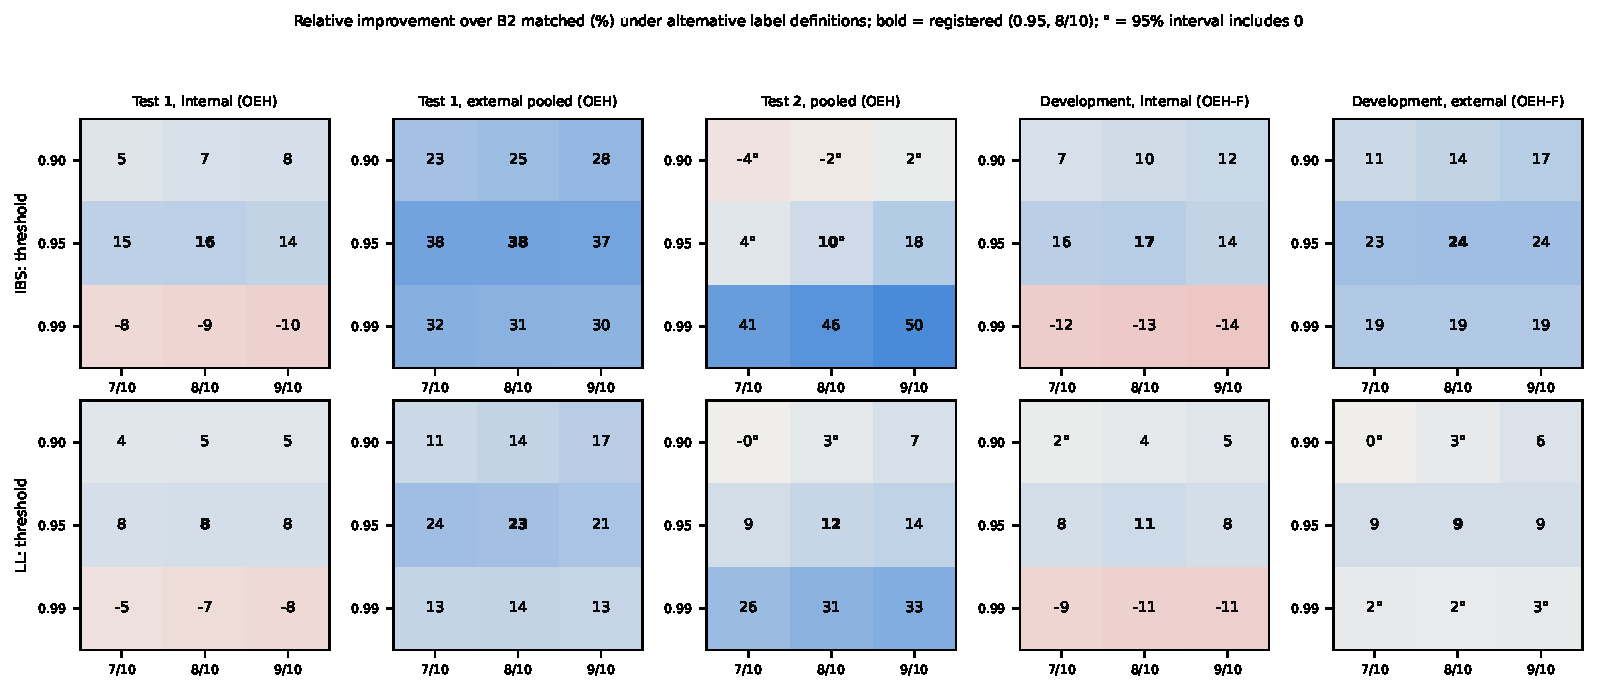
\includegraphics[width=\textwidth]{figures/fig_threshold_sensitivity.pdf}
\caption{Relative improvement over B2 matched (\%) of the sealed forecasts under alternative label definitions (rows: $\tau$; columns: successful seeds out of ten). Bold: registered definition; $^\circ$: 95\% interval includes zero.}
\label{fig:threshold-sensitivity}
\end{figure*}
